\documentclass[crop,tikz,convert={outext=.svg,command=\unexpanded{pdf2svg \infile\space\outfile}},multi=false]{standalone}
\usepackage{amsmath}
\usepackage{amssymb}
\usepackage{mathtools}
\usepackage{fullpage}
\usepackage[T1]{fontenc}
\usepackage{lmodern}
\usepackage{tikz}
\usetikzlibrary{calc,intersections,through,backgrounds}
\usetikzlibrary{bayesnet}
\usepackage{tikzscale}
\usepackage{tkz-euclide}
\usepackage{tcolorbox}
\tcbuselibrary{skins,breakable}
% pgfplots
\usepackage{pgfplots}
\pgfplotsset{compat=1.8}
% For entities in text
\newcommand{\entity}[1]{\texttt{#1}}
% For entities in pgfplots
\newcommand{\entpgf}[1]{\texttt{#1}}
	
\begin{document}
	
	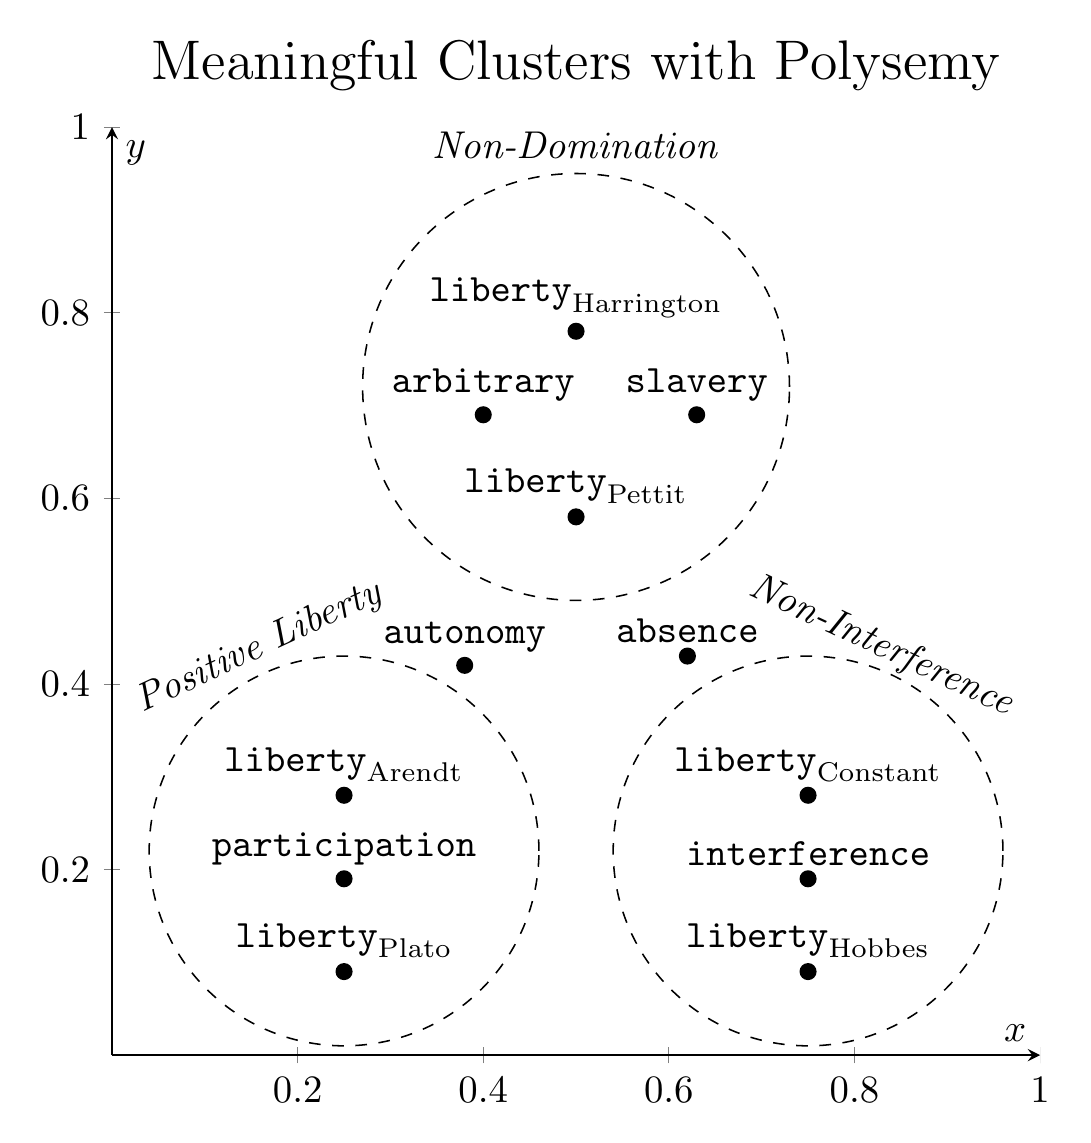
\begin{tikzpicture}[scale=1.4]
		\begin{axis}[axis lines=center,
			title={\Large Meaningful Clusters with Polysemy},
			%view={28}{22},
			xmin=0, xmax=1, ymin=0, ymax=1,
			%xtick={0,1},ytick={0,1.0},
			xlabel=$x$,ylabel=$y$,width=10cm,height=10cm]
			\addplot+[mark options={fill=black,color=black},only marks,point meta=explicit symbolic, nodes near coords] coordinates 
			{
				% top left: withdrawal_drugs
				(0.5,0.78)[$\texttt{liberty}_\text{Harrington}$]
				(0.5,0.58)[$\texttt{liberty}_\text{Pettit}$]
				(0.4,0.69)[$\texttt{arbitrary}$]
				(0.63,0.69)[$\texttt{slavery}$]
				% bottom left: bank_money
				(0.25,0.28)[$\texttt{liberty}_\text{Arendt}$]
				(0.25,0.09)[$\texttt{liberty}_\text{Plato}$]
				(0.25,0.19)[$\texttt{participation}$]
				(0.38,0.42)[$\texttt{autonomy}$]
				% top right: bank_water
				% waves
				%(0.8,0.8)[{\includesvg[width=5.5mm]{./ch0/figs/1F30A.svg}}]
				% droplet
				(0.62,0.43)[$\texttt{absence}$]
				(0.75,0.28)[$\texttt{liberty}_\text{Constant}$]
				(0.75,0.09)[$\texttt{liberty}_\text{Hobbes}$]
				(0.75,0.19)[$\texttt{interference}$]
				% bottom right: stream_music
				% 3 notes
				%(0.8,0.19)[{\includesvg[width=5.5mm,height=5.5mm]{./ch0/figs/1F3B6.svg}}]
				% 1 note
				%(0.8,0.3)[$\textsf{stream}_2$]
			};
			%\addplot+ graphics[xmin=0,xmax=96,ymin=0,ymax=96] {Dad64.png};
			% Positive Liberty + Circle
			\node[rotate=25] (a) at (axis cs:0.16,0.44) {\textit{Positive Liberty}};
			\draw[dashed] (axis cs:0.25,0.22) circle [blue, radius=0.21];
			\node[rotate=-25] (a) at (axis cs:0.83,0.44) {\textit{Non-Interference}};
			\draw[dashed] (axis cs:0.75,0.22) circle [blue, radius=0.21];
			% Non-Domination + Circle
			\node[] (a) at (axis cs:0.5,0.98) {\textit{Non-Domination}};
			\draw[dashed] (axis cs:0.5,0.72) circle [blue, radius=0.23];
		\end{axis}
	\end{tikzpicture}

\end{document}
